\section{基于LSTM进行汽车位置预测的GNSS位置欺骗攻击检测模型}
\subsection{模型概述}
如\ref{sec:LSTM_gaishu}所述,LSTM作为传统RNN的改进模型,可以解决长序列问题中长期依赖的问题。对于本文中所涉及到的GNSS位置欺骗检测问题,由于汽车的移动轨迹可以看作是一个有依赖关系的连续序列,因此,可以使用LSTM作为问题的解决方案。模型的检测思路为,以被欺骗前目标车辆的CAN速度、IMU前向加速度以及转向角作为输入,输出为下一时刻目标车辆所处位置与当前车辆位置之间距离的预测值$dis_p$。计算$dis_p$与车辆实际移动距离$dis_g$的绝对值$dis_{abs}$,并设置欺骗阈值$\gamma$。若满足$dis_{abs}>\gamma$,则认为此时目标车辆受到了GNSS位置欺骗。$\gamma$的定义如下:
\begin{equation}
    \gamma=\epsilon_{GNSS}+\epsilon_{LSTM}
    \label{eq:gamma}
\end{equation}
其中,$\epsilon_{GNSS}$表示汽车GNSS模块定位误差,$\epsilon_{LSTM}$表示检测模型的预测误差。
本文所使用的模型结构包括输入层、包含50个神经元的隐藏层以及输出层。如图\ref{fig:my_model_arch}所示。
\begin{figure}[htbp]
    \begin{center}
        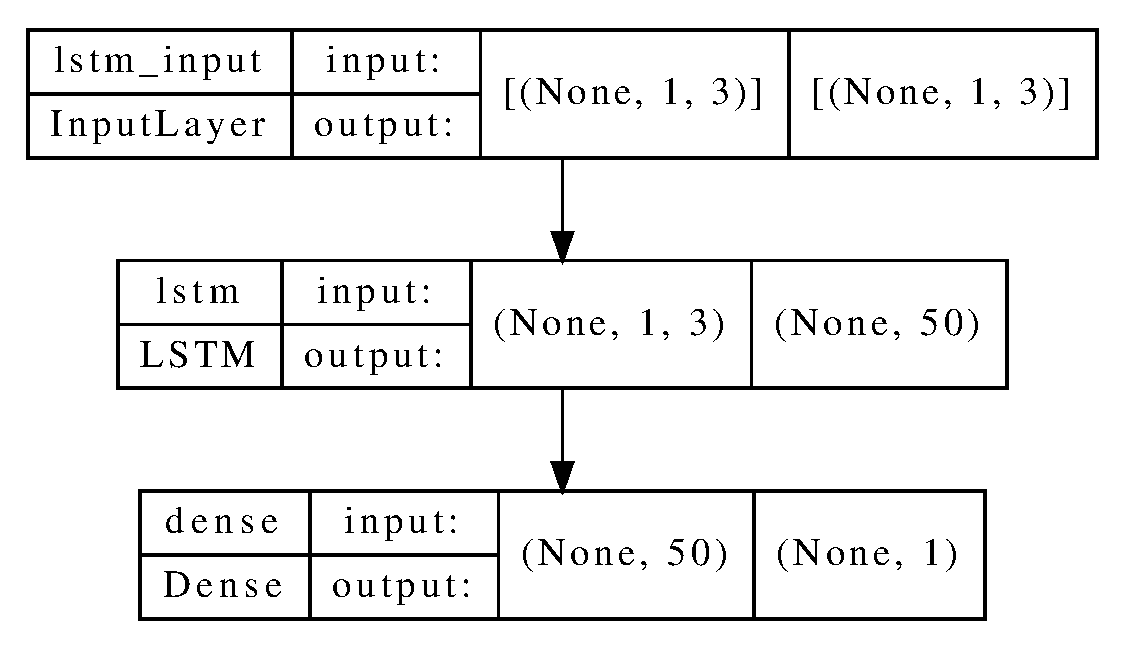
\includegraphics[width=0.8\textwidth]{LSTM.eps}
    \end{center}
    \caption{本文所使用的LSTM模型结构}
    \label{fig:my_model_arch}
\end{figure}

\subsection{模型训练}
本文在模型训练过程中将学习率设置为0.01,batch size设置为64,并使用Adam优化器。另外,使用平均绝对误差(Mean Absolute Error,MAE)作为损失函数。MAE的定义如\ref{eq:MEA}所示。
\begin{equation}
    MAE=\frac{1}{N}\sum_{i=1}^N|y_p-y_g|
    \label{eq:MAE}
\end{equation}
其中,$N$表示总样本数目,$y_p$与$y_g$分别表示模型预测距离以及真实距离。
\subsection{本章小结}
